\chapter{Projekt OpenStreetMap}
\section{O~projektu}
Projekt OpenStreetMap \cite{osmweb} vznikl v~Anglii v~roce 2004 a jeho prvotním cílem bylo
vytvořit volně dostupná geografická data pro Velkou Británii. Iniciativa se
postupně rozrostla do celého světa a dnes mapu pomáhá tvořit přes milion
dobrovolníků. Česká republika je dnes poměrně kvalitně pokryta a zvláště velká
města mají dostatečně detailní pokrytí i pro vyhledávání pěších tras.

\section{Datová primitiva} 
Projekt OpenStreetMap používá tři základní geografická primitiva: uzly, cesty a
relace. Ke každému z~těchto primitiv mohou být přiřazeny atributy, což jsou
dvojice klíče a hodnoty. Každý typ primitiv má svou číselnou řadu, ze které
dostává každý prvek unikátní číslo v rámci této řady -- id. 
U~polohových dat se neukládá výška, výsledná mapa je pouze dvourozměrná.
Nyní popíšeme jednotlivá primitiva:

{\tuc Uzly} jsou body s~určenými souřadnicemi. Uzly mohou mít atributy, ty pak
určují bodový mapový objekt, například rozcestník nebo závoru. Existují i uzly
bez atributů sloužící pouze jako součást cest nebo relací.

{\tuc Cesty} jsou lomené čáry definované posloupností uzlů. Uzly se na cestě nemohou opakovat
s~jedinou výjimkou: první a poslední bod mohou být shodné, potom se jedná
o~uzavřenou cestu. Cesty jsou orientované, tzn. na pořadí uzlů záleží. Mohou
existovat cesty bez atributů jako součásti relace, ale obvykle mají atributy
určující, jaký objekt reálného světa popisují.

Pomocí cest popisujeme linie a plochy. Pokud má být cesta plochou, musí být
uzavřená, ale ne každá uzavřená cesta je plocha. Tento problém rozebíráme níže.
Jedna cesta také může reprezentovat více fyzických objektů (například silnici
s~tramvajovou tratí, park s~oplocením).

{\tuc Relace} jsou posloupnosti uzlů a cest opatřené atributy. Každý prvek
v~relaci navíc může mít určenou roli. Relace může obsahovat jako prvek i relaci,
ale tato situace není příliš dobře podporována programy pracujícími s daty OSM. 
Obvykle jsou relacemi reprezentovány složitější objekty, které by se cestami a
uzly popisovaly obtížně, nebo také \uv{virtuální} objekty jako například
trasy linek MHD, cyklotrasy a územní hranice.

Pro nás důležitý typ relace je {\tuc multipolygon}, který se používá k~reprezentaci
složitějších ploch. Plocha reprezentovaná multipolygonem se může skládat z více
nesouvisejících částí nebo obsahovat díry. Multipolygon obsahuje cesty s~rolemi 
\verb|INNER| resp. \verb|OUTER| indikující, zda je cesta součástí vnější resp.
vnitřní hranice plochy. Hranice multipolygonu se mohou skládat z více částí, ale
vždy musí dohromady tvořit jednu nebo několik uzavřených částí tvořících obvody 
plochy resp. díry v ploše.

\section{OSM XML}
Nejobvyklejší způsob ukládání OSM dat je ve formátu XML. Všechna primitiva mají
jako jeden z~atributů \verb|id|, který značí jejich jednoznačný identifikátor.
Každý typ primitiva má svou vlastní číselnou řadu. V~OSM XML \cite{osmxml} je
nejprve hlavička, následně seznam uzlů, seznam cest a seznam relací. Níže je
příklad takového souboru, za ním následuje popis jednotlivých částí souboru.

% Pozor na zlom stránky
\begin{verbatim}
<!-- Hlavička -->
<?xml version='1.0' encoding='UTF-8'?>
<osm version="0.6" generator="osmconvert 0.7T">
	<bounds minlat="49.4645" minlon="14.334" maxlat="49.466" 
	maxlon="14.339"/>

<!-- Uzly -->
	<node id="962931066" lat="49.4647188" lon="14.3384903" version="1" 
	timestamp="2010-10-24T05:47:30Z" changeset="6153364" uid="1066" />

<!-- Cesty -->
	<way id="82704082" version="1" timestamp="2010-10-24T06:27:17Z" 
	changeset="6153364" uid="1066" user="pavel">
	    <nd ref="962425008"/>
	    <nd ref="962931066"/>
	    <nd ref="962738699"/>
	    <nd ref="962425008"/>
	    <tag k="dibavod:id" v="9890"/>
	    <tag k="natural" v="wetland"/>
	    <tag k="source" v="dibavod A06"/>
	</way>

<!-- Relace -->
	<relation id="25793" version="3" timestamp="2012-07-31T09:21:12Z" 
			changeset="12558592" uid="82083" user="petr_balicek">
	    <member type="way" ref="26082949" role="outer"/>
	    <member type="way" ref="26080423" role="inner"/>
	    <member type="way" ref="26080424" role="inner"/>
	    <tag k="landuse" v="forest"/>
	    <tag k="type" v="multipolygon"/>
	</relation>
	<relation id="2331090" version="3" timestamp="2012-10-03T21:29:24Z"
			changeset="13353948" uid="8007" user="vrabcak">
	    <member type="way" ref="174291392" role=""/>
	    <tag k="boundary" v="protected_area"/>
	    <tag k="leisure" v="nature_reserve"/>
	    <tag k="name" v="PP Boukal"/>
	    <tag k="type" v="boundary"/>
	</relation>
</osm>
\end{verbatim}

{\tuc Hlavička souboru.} V~XML hlavičce je určeno kódování UTF-8 a následně je
otevřen element \verb|osm|. 

{\tuc Uzly.} Zde jsou za sebou postupně vypsány všechny uzly.  Pro uzly
používáme element \verb|node|. Každý uzel má atributy \verb|lat| a \verb|lon|
určující jejich zeměpisnou šířku a délku; používá se souřadný systém
WGS-84. \cite{wgsnorma} Dále mohou mít vnořené elementy \verb|tag|. Každý tento
element má atribut \verb|k| a \verb|v| definující pár (klíč,hodnota), který
popisuje vlastnosti uzlu.

{\tuc Cesty.} Zde jsou za sebou vypsány cesty. Cesty jsou reprezentovány
elementem \verb|way|, v~němž jsou vnořeny elementy \verb|nd|. Každý element
\verb|nd| reprezentuje odkaz na jeden uzel na cestě, identifikátor tohoto uzlu
je uložen v~atributu \verb|ref|. Také cesty mohou mít vnořené elementy
\verb|tag|.

{\tuc Relace.} Jako poslední jsou vypsány všechny relace, reprezentované
elementem \verb|relation|. Prvky relací jsou reprezentovány elementy
\verb|member|, které obsahují atributy \verb|type| určující, o~jaký typ
primitiva jde, \verb|ref| určující identifikátor tohoto primitiva a \verb|role|
určující roli daného prvku v~relaci. I~relace mohou mít vnořené elementy
\verb|tag|.

Toto pořadí umožňuje proudově zpracovávat XML, protože když zpracováváme cesty,
tak již máme v~paměti všechny uzly, na které se cesty mohou odkazovat, obdobně
s~relacemi. Problém může nastat, pokud je relace prvkem relace. Pak není
uspořádání definováno, ale obvykle je dodržováno. 

OSM XML se dá volně stáhnout, většinou jsou tyto soubory pro úsporu místa
zkomprimované a aktualizují se jednou denně. Protože většina aplikací
nepotřebuje data z~celého světa, jsou k~dispozici i data pro jednotlivé
kontinenty a státy.\footnote{\url{http://osm.kyblsoft.cz/archiv/}}

\section{Problémy v~datech}
Ačkoli jsou data z~OSM poměrně kvalitní a přesná, během jejich zpracování jsme
narazili na některá problematická místa. 

{\tuc Různorodé označování ploch.} Tento problém plyne již z~definice geografických
primitiv a atributů objektů. Protože jak plochy, tak linie jsou označovány v~OSM
stejným primitivem cesta, musí se při rozlišování hledět na jejich atributy.
Bohužel ani zde není jejich používání sjednoceno. Aby mohla být cesta
plochou, musí mít první a poslední uzel stejný. Ale ne každá uzavřená 
cesta je plochou. Například uzavřená silnice se pokládá za kruhový objezd a
nikoli za plochu. Aby byla považována za plochu, musí mít nastaven klíč
\verb|area| hodnotu \verb|yes|. Naopak pokud má cesta například klíč \verb|landuse|
nebo \verb|building|, je za plochu považována, i když nemá klíč \verb|area|.

\smallskip
{\tuc Nekorektní objekty.} I~přesto, že editory používané pro úpravu OSM se snaží
hlídat správnost vytvořených objektů, se v~mapě vyskytují různé chybně
definované objekty. Nalezli jsme například cesty, které samy sebe kříží,
chybějící elementy v~hranicích multipolygonu a jiné. Výhodou OSM je, že jsme je
mohli ihned opravit, ale přesto je musí umět program korektně vyhodnotit.

\smallskip
{\tuc Více bodů na stejných souřadnicích.} Ač by se pro spojování sousedních
ploch měly využívat společné body na hranicích, v~některých oblastech jsme našli
problematická místa, kde polovina ploch používala jeden bod a druhá polovina
jiný na stejných souřadnicích. Tyto dva body spolu nebyly nijak propojeny a
pravděpodobně vznikly při některém importu z~jiných datových zdrojů. Takovýchto
chyb jsme nalezli mnoho a je opět potřeba je korektně zpracovat.

\smallskip
{\tuc Různá sémantika atributů na různých místech.} Při výběru atributů, které
zahrnout ke zpracování, jsme se setkali s~používáním stejných atributů v~různých
významech. Například klíč \verb|landuse| s~hodnotou \verb|residential| má dle
specifikace \cite{osmfeatures} označovat obytnou oblast. V některých místech
jsou tímto klíčem a hodnotou označena přístupná prostranství mezi budovami. 
Kvůli těmto nejednoznačnostem jsme některé atributy nemohli použít, protože by
vytvářely v~některých částech města nekorektní výsledky.
\begin{figure}
	\centering
	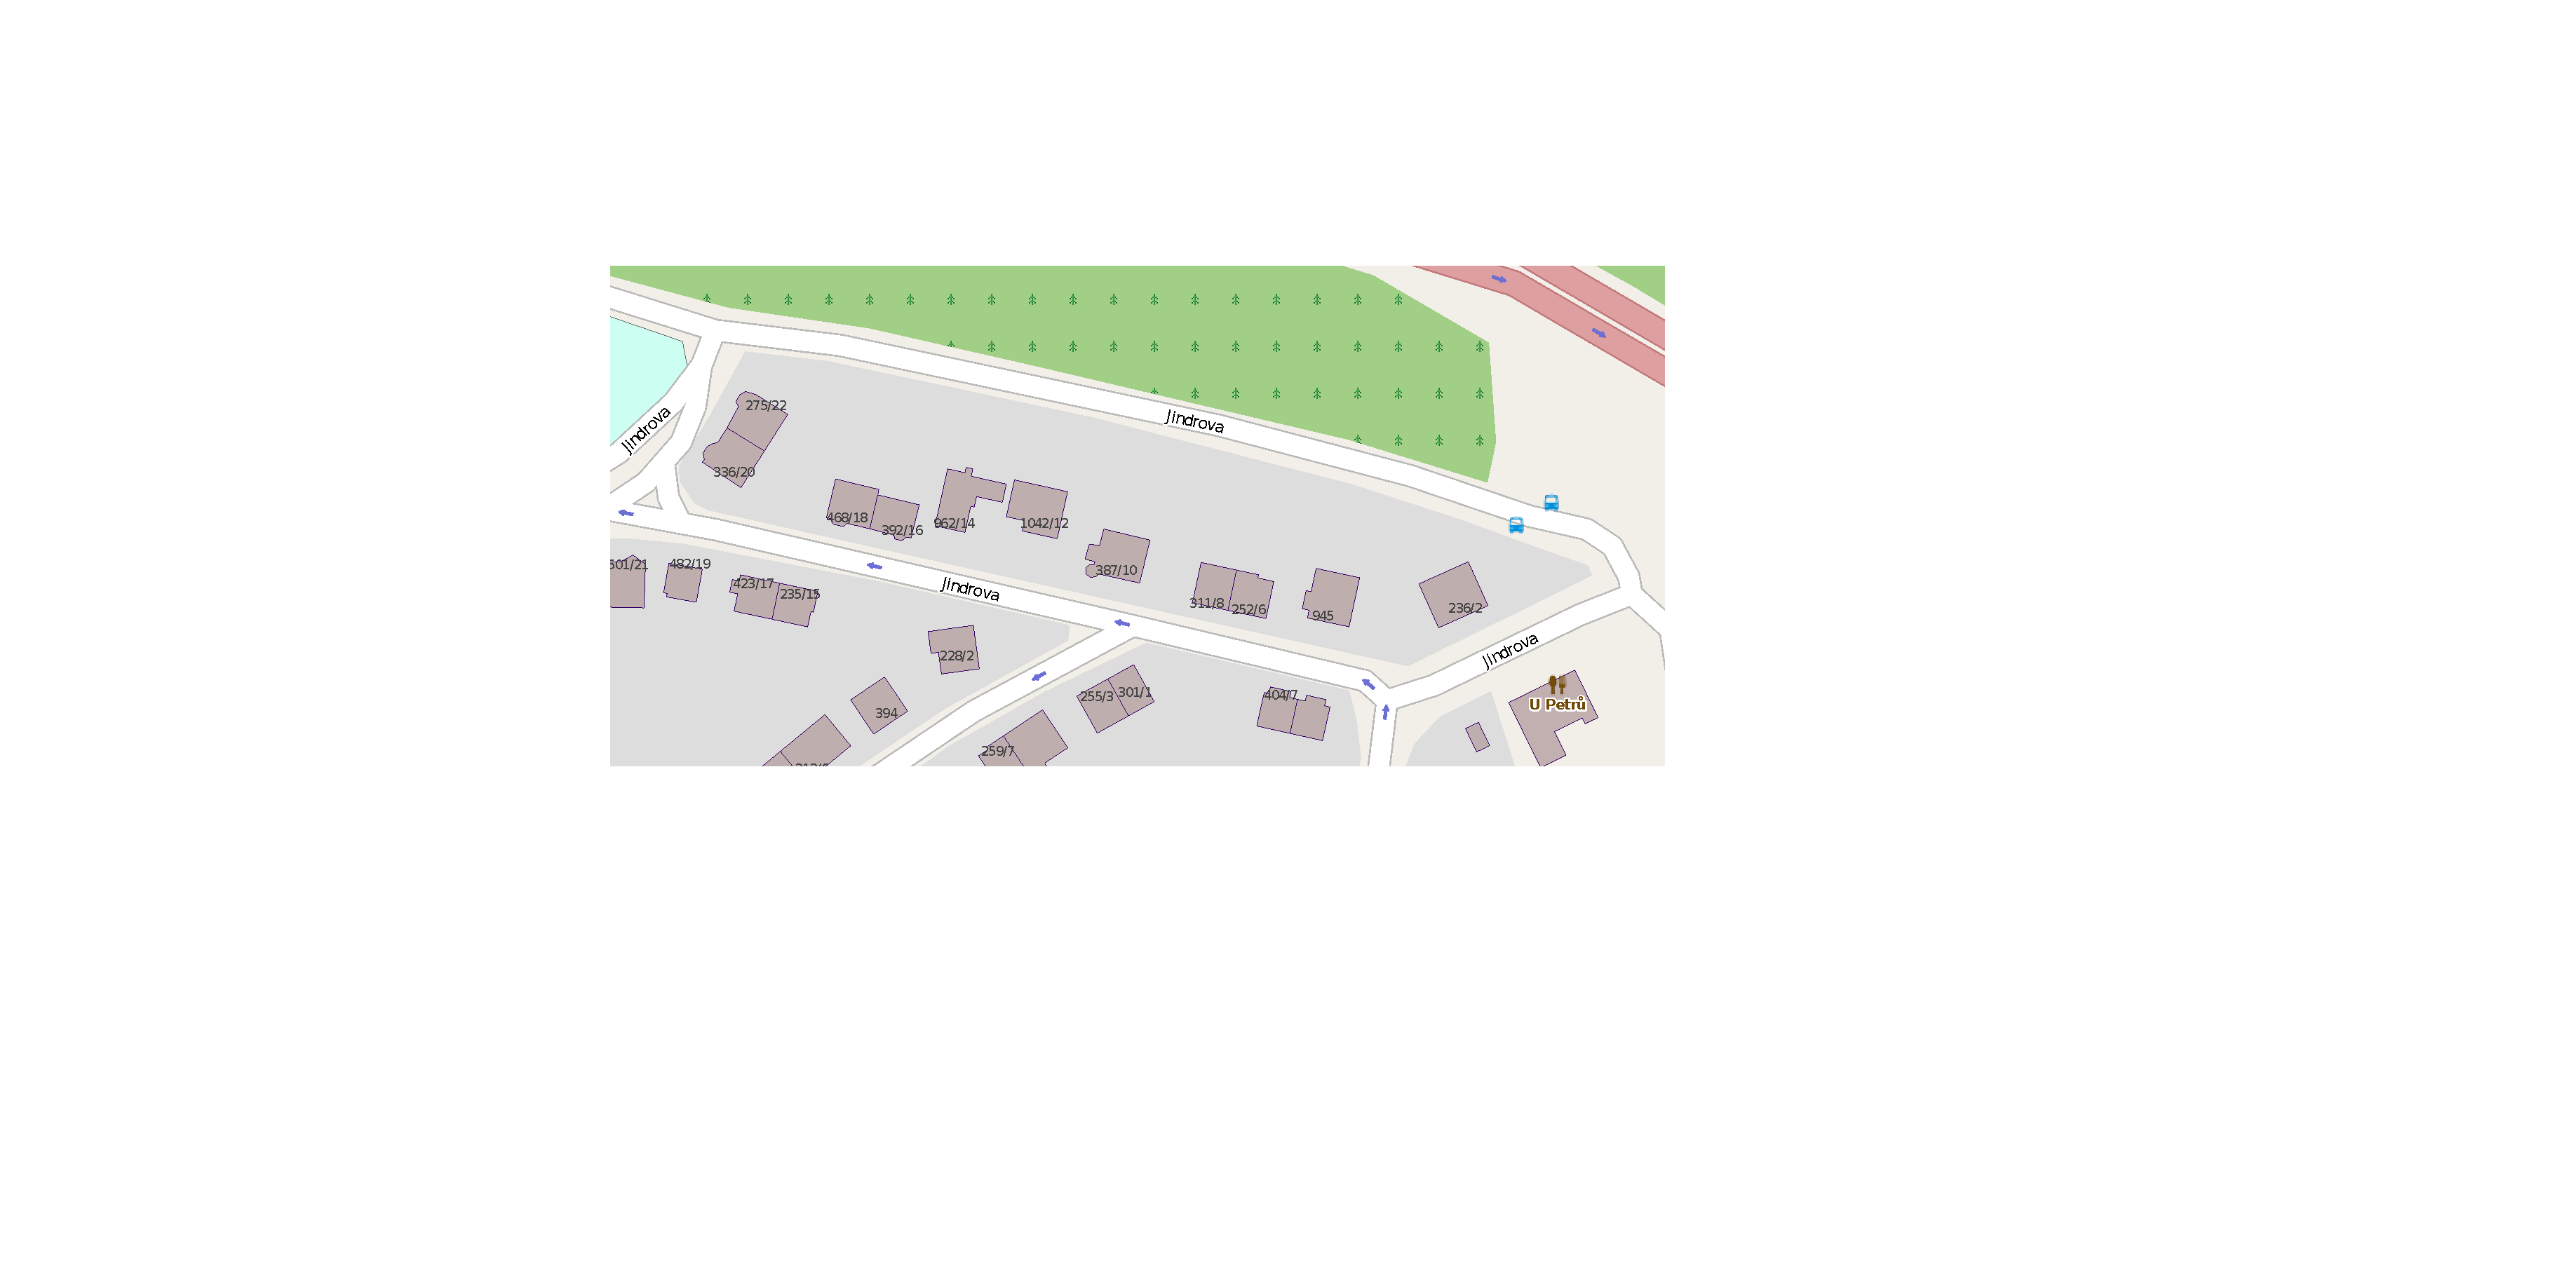
\includegraphics[width=80mm]{../img/resident-nepruch.pdf}
	\caption{\texttt{landuse=residential} jako označení oplocených rodinných
	domků je správně dle specifikace.}
	\label{fig:resident-nepruch}
\end{figure}
\begin{figure}
	\centering
	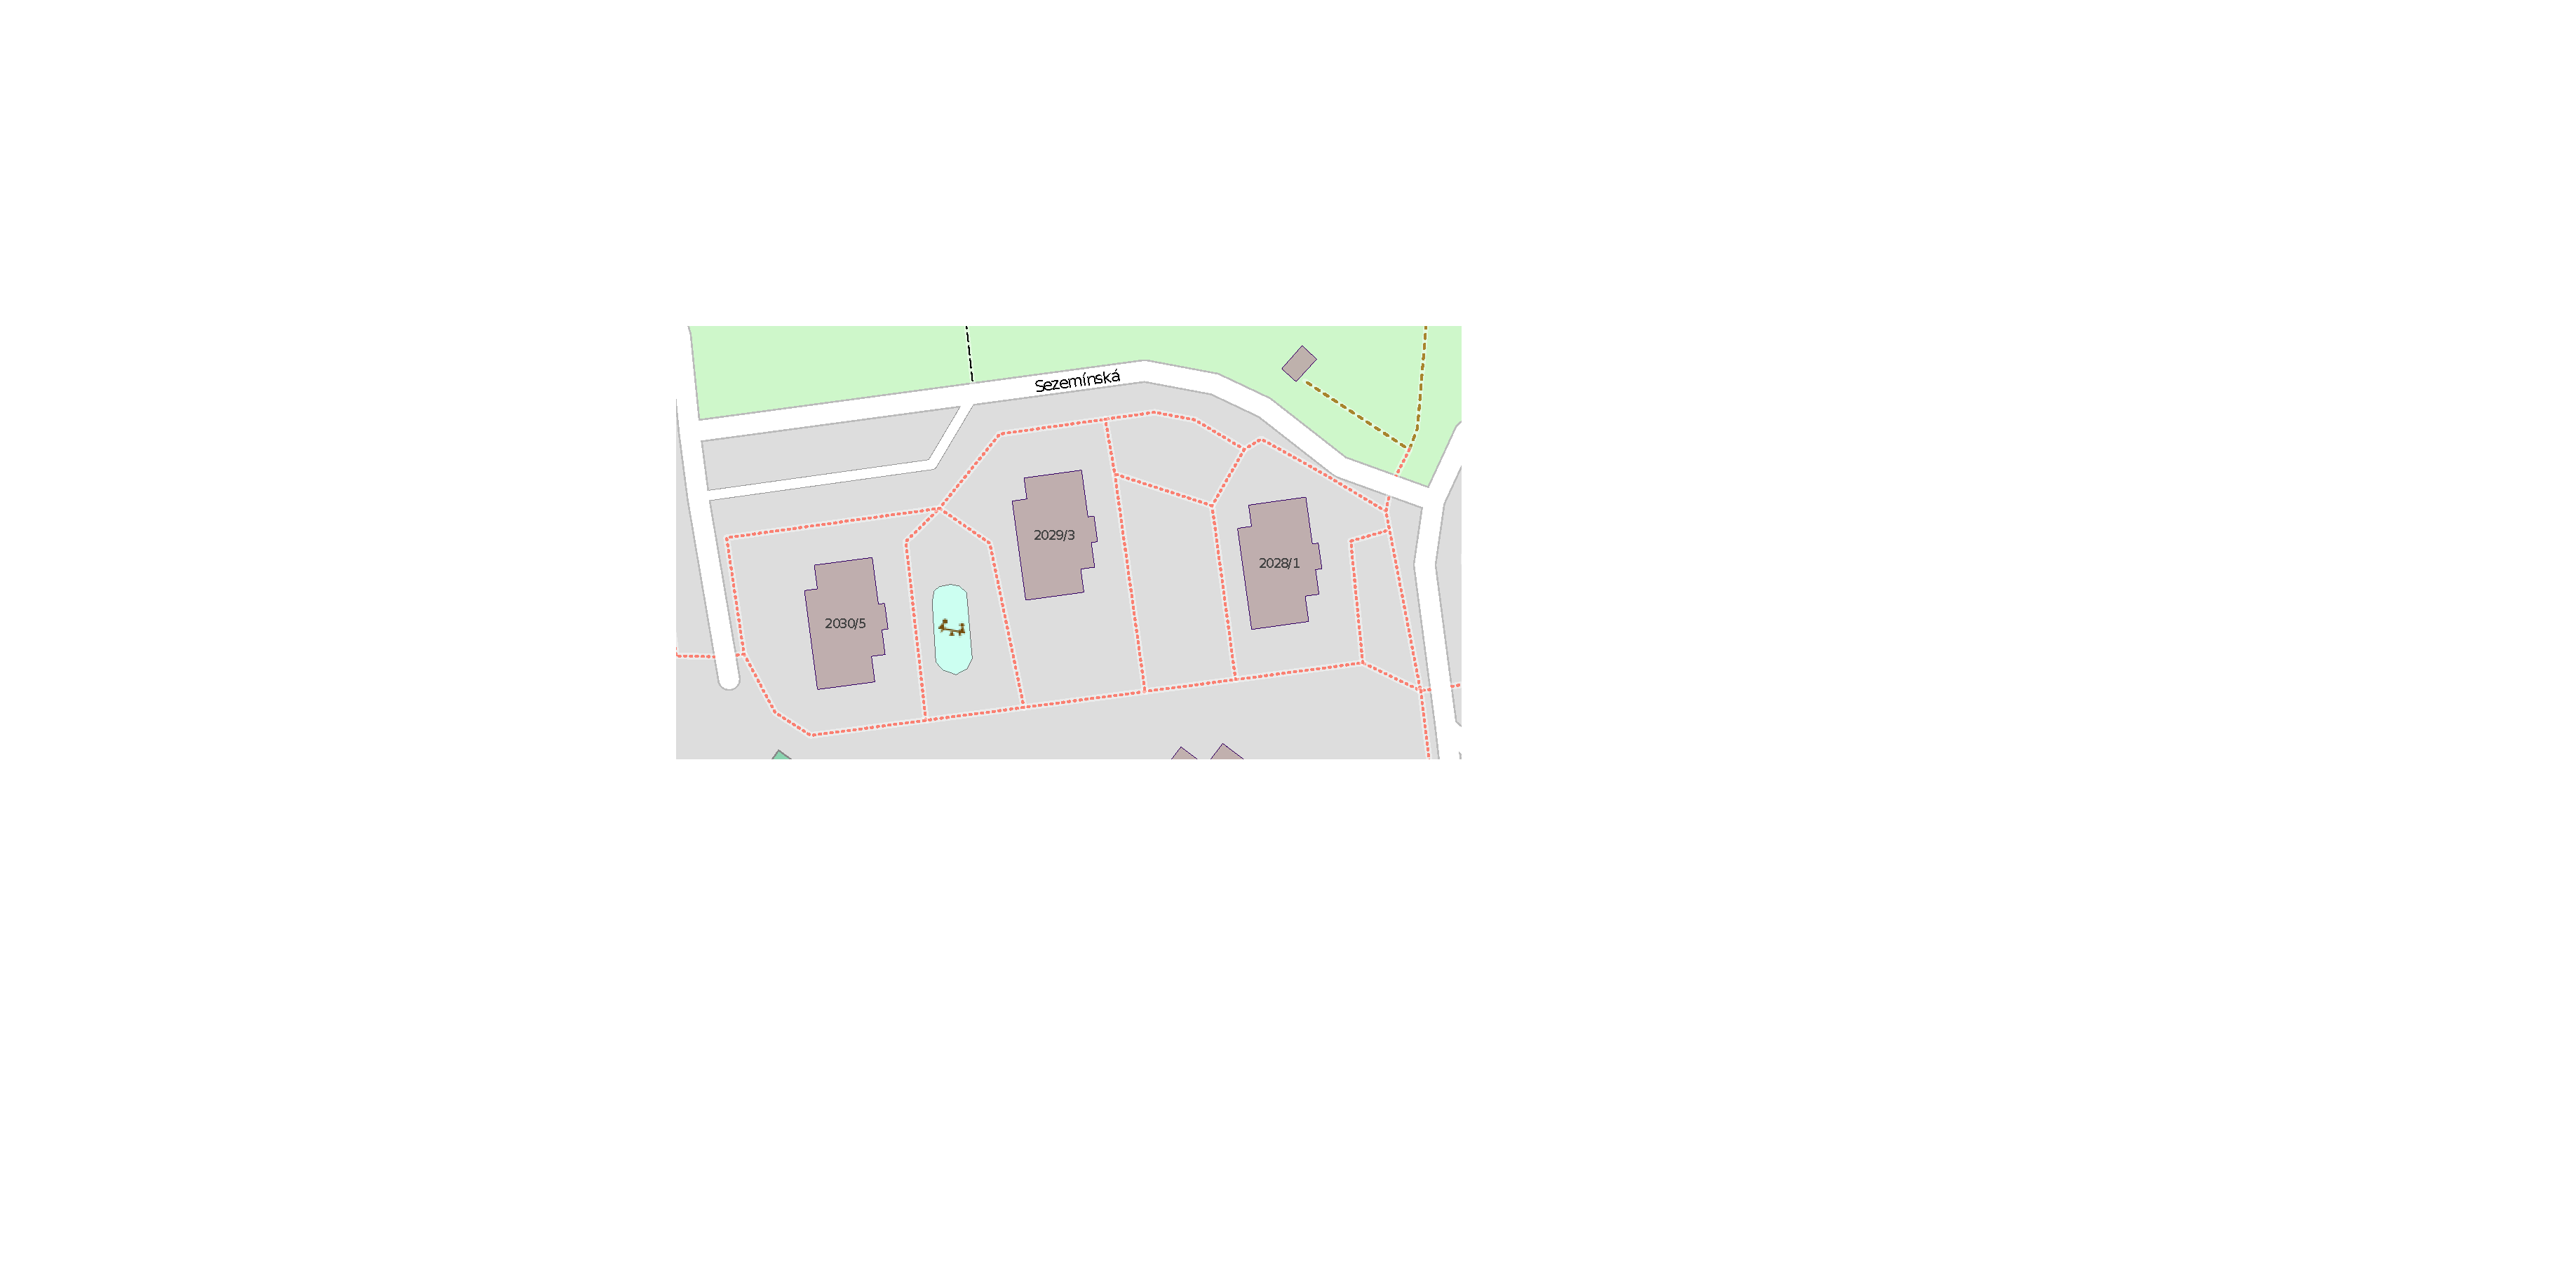
\includegraphics[width=80mm]{../img/resident-plocha.pdf}
	\caption{\texttt{landuse=residential} jako označení průchozí plochy mezi
	paneláky. Také jde o správné označení dle specifikace (jedná se o
	obytnou zástavbu), ale navíc by bylo vhodné označit přesněji plochu, aby
	bylo zřejmé, že je průchozí a dají se na ní hledat trasy i mimo cesty.}
	\label{fig:resident-volno}
\end{figure}

{\tuc Neúplně navazující cesty.} Kvalita mapovaných cest v~OSM je silně závislá na typu
cesty. Zatímco silnice, které jsou často využívány pro hledání tras, jsou
většinou navzájem navázány správně, chodníky často v~datech úplně chybí, nebo
nejsou napojeny na silnice. Rovněž přechody často chybí. Proto v~našem programu
zkoumáme i okolí cest a přidáváme možné spojky mezi chodníky a silnicemi.
\begin{figure}
	\centering
	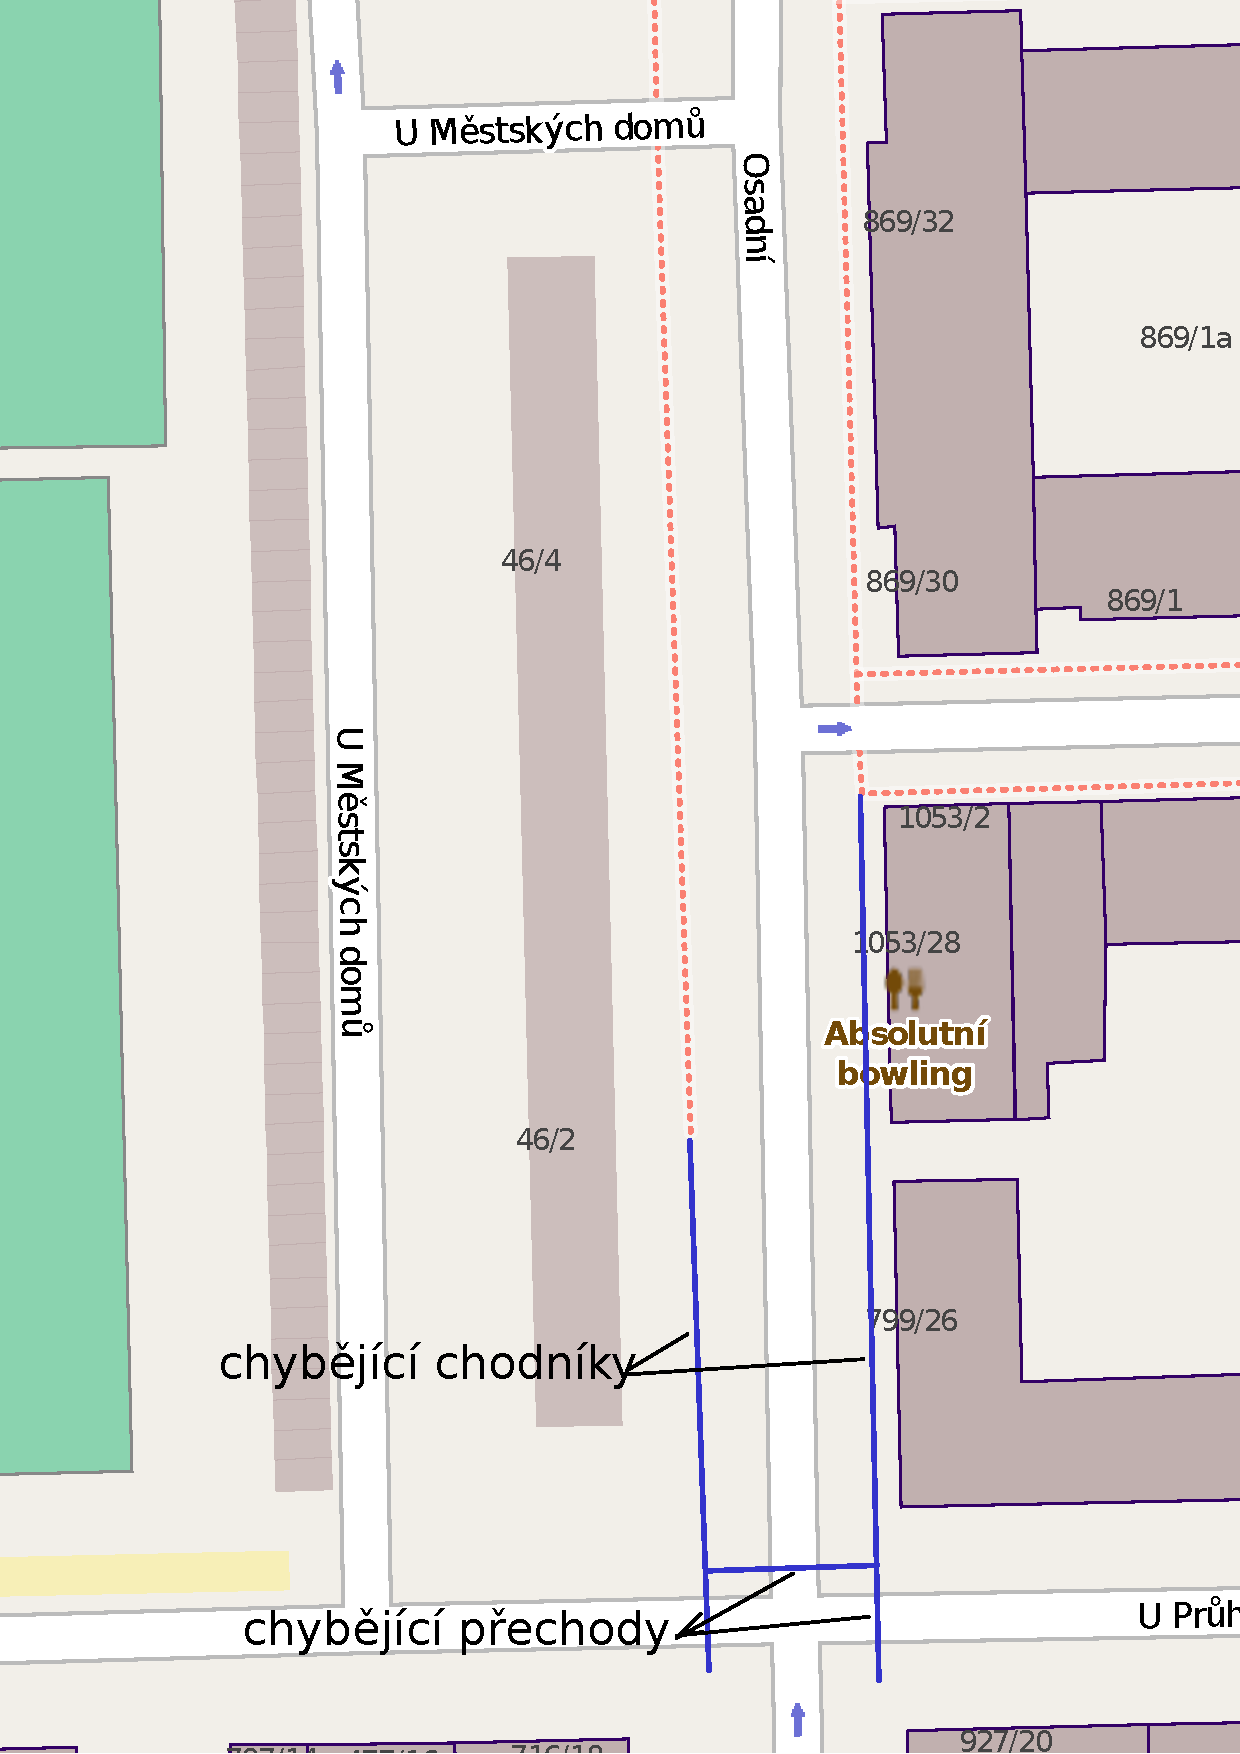
\includegraphics[width=50mm]{../img/chodnik.pdf}
	\caption{Špatně zmapovaný chodník. Chodník ve skutečnosti vede po obou
	stranách ulice Osadní, na křižovatce dole jsou přechody přes všechna
	její ramena.}
	\label{fig:chodnik}
\end{figure}

\section{Využívané informace z~OSM}
Protože chceme umět nejen vyhledávat po cestách, ale i vytvářet trasy přes
průchozí prostranství, potřebujeme mimo cest zpracovávat i budovy, prostranství 
a další objekty. Zpracováváme cesty, které popisují fyzické objekty v~terénu,
naopak vynecháváme správní hranice, podzemní objekty (např. metro) a cesty
popisující služby a občanskou vybavenost. Uzly zpracováváme jen jako body
s~danou polohou, jejich atributy nevyužíváme. Z~relací používáme pouze
multipolygon, kterým jsou často reprezentovány budovy.

